%----------------------------------------------------------------------------
\chapter{A generált monitor forráskód helyességének tesztelése}
%----------------------------------------------------------------------------

%----------------------------------------------------------------------------
\section{Tesztelési célok}
%----------------------------------------------------------------------------

A generált monitor forráskód tesztelésére a következő célokat fogalmazzuk meg:

\begin{itemize}
    \item Az összes üzenet típus megjelenése a különböző teszt szcenáriókban
    \item Időzített feltételek helyes kiértékelése
    \item Üzenet megkötések tesztelése
    \item \textit{Alt} és \textit{Par} operátorok esetén, az üzenet szekvencia ágak helyes kiértékelése
    \item \textit{Loop} operátor esetén a minimális és maximálás üzenet ismétlődések tesztelése
    \item Összetett szcenárió tesztelése, ami több operátort tartalmaz
    \item Egymást követő elvárt üzeneteket tartalmazó szcenárió tesztelése
    \item Egymást követő \textit{fail} üzeneteket tartalmazó szcenárió tesztelése
    \item \textit{Regular} üzenet tesztelése (ha megjelenik a rendszer működésében, akkor ki kell értékelni a szcenárió többi részét, ha nem jelenik meg, a monitor helyes működést kell jelezzen és, hogy a követelmény nem teljesült)
    \item Több óraváltozót tartalmazó szcenárió tesztelése
    \item Egymást követő különböző típusú üzenetek kombinációinak tesztelése (pl. elvárt üzenetet követő \textit{fail}, elvárt üzenetet követő reguláris, stb.)
\end{itemize}

%----------------------------------------------------------------------------
\clearpage\section{Monitor forráskód generátor tesztelése}
%----------------------------------------------------------------------------

Egy teszt bemenetként egy \textit{TPSC} leírást, egy szimulált esemény szekvenciát és egy elvárt kimenetet fog kapni.
A tesztelt monitornak kézzel küldünk üzeneteket, konkrét esemény lefutását.
A monitor kimenetét összehasonlítjuk az elvárt kimenettel, amelyet kézzel állítunk össze figyelembe véve, hogy a szimulált rendszer működésének elméletben meg kell-e felelnie a követelménynek vagy sem.
Ez két információt tartalmaz, hogy a rendszer jó állapotban van-e és teljesíti-e a követelményt.
Ha egyezik akkor sikeres a teszt, ellenkező esetben pedig sikertelen.

\begin{figure}[!ht]
    \centering
    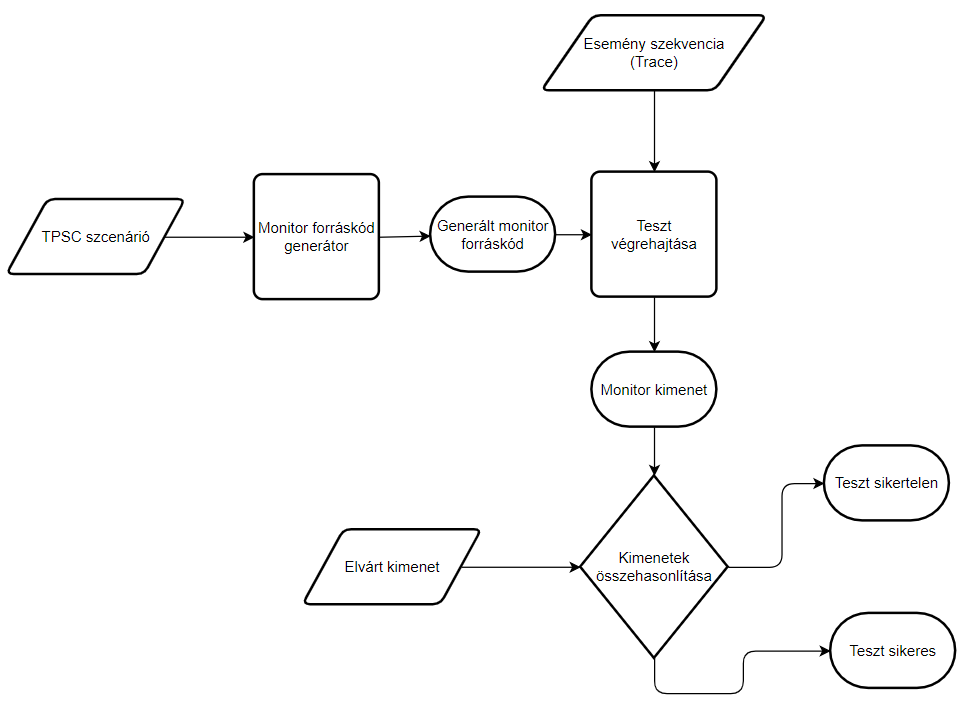
\includegraphics[width=160mm, keepaspectratio]{figures/test_flowchart.png}
    \caption{Tesztelés folyamatábrája.}
    \label{testing_figure}
\end{figure}

Az \textit{Xtext} keretrendszer a specifikált \textit{DSL (Domain Specific Language)} nyelvhez generál egy \textit{Maven} \cite{Maven} \textit{plugin}-t.
Ezt a \textit{plugin}-t betölthetjük egy egyszerű \textit{Maven} projektbe és használhatjuk is az elkészített \textit{DSL} nyelvünket, azaz létrehozhatunk a projektben a saját \textit{DSL}-ünkhöz tartozó fájlokat, melyekben megadhatjuk saját szcenárióinkat.

Az esemény szekvenciában lévő üzeneteket a monitor \textit{update()} függvényénét használva adjuk át neki.
A teszteset végén pedig a \textit{JUnit} tesztelési keretrendszer \textit{Assertions} osztályát használjuk, hogy a monitor kimenetét összehasonlítsuk az elvárt kimenettel.
A teszteredmény ennek az összehasonlításnak az eredménye lesz.

A \ref{testing_figure} ábrán megtekinthető a tesztelés tervének folyamatábrája.

%----------------------------------------------------------------------------
\clearpage
%----------------------------------------------------------------------------

Az \textit{Xtext} keretrendszer által nyújtott \textit{Maven plugin}-t felhasználhatjuk a tesztjeinkhez.
Elég csupán egy \textit{Maven} projektet felkonfigurálni a saját \textit{DSL plugin}-ünkkel és elkészíthetjük a saját tesztelési keretrendszerünket.
A keretrendszerünk tartalmazza a tesztszcenárióhoz készített \textit{TPSC} szöveges leírásának a fájlját, a monitor forráskód generátort \textit{Maven plugin} formájában és egy \textit{Java} osztályt, amely a teszteseteket tartalmazza.
Ezen kívül függőségként még be kell töltenünk a \textit{util} csomagot, hogy hozzáférhessünk a monitor statikus forráskódjához is.
Ezek a \textit{Maven} projektek a szülő projektünkben helyezkedhetnek el, így a projekt struktúrában közvetlen a nyelvünk mellett vannak.
A \ref{integration_test_structure} ábrán látható egy ilyen teszthez tartozó \textit{Maven} projekt felépítése

\begin{figure}[!ht]
    \centering
    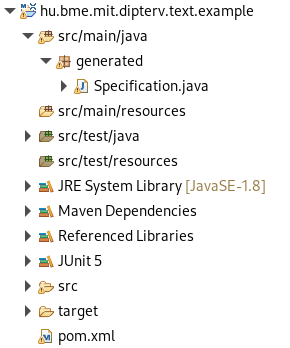
\includegraphics[width=100mm, height=7cm, keepaspectratio]{figures/test_example_structure.png}
    \caption{Példa \textit{Maven} teszt projekt struktúrája.}
    \label{integration_test_structure}
\end{figure}

A \ref{integration_test_structure} ábrán lévő \textit{generated} csomag tartalmazza a szcenárióhoz tartozó generált automata forráskódját.

\begin{lstlisting}[language=java, frame=single, float=ht!, caption={Teszteset eredménye.},captionpos=b,label=maven_test_output]
-------------------------------------------------------
T E S T S
-------------------------------------------------------
Running hu.bme.mit.dipterv.text.example.MonitorPassingTest
q0 NORMAL
q1 NORMAL
q2 ACCEPT
q3 NORMAL
q4 NORMAL
q5 FINAL
!(computer.checkEmail().computer) q0->q0
computer.checkEmail().computer q0->q1
!(computer.sendUnsentEmail().server) q1->q1
!(computer.sendUnsentEmail().server) q1->q2
computer.sendUnsentEmail().server q1->q3
!(computer.logout().server) & !(computer.newEmail().server) q3->q3
computer.newEmail().server q3->q4
!(computer.downloadEmail().server) q4->q4
computer.downloadEmail().server q4->q5
Received Message: computer.checkEmail().computer
Transition: !(computer.checkEmail().computer)
Transition: computer.checkEmail().computer
transition triggered: computer.checkEmail().computer
q1

Received Message: computer.sendUnsentEmail().server
Transition: !(computer.sendUnsentEmail().server)
Transition: !(computer.sendUnsentEmail().server)
Transition: computer.sendUnsentEmail().server
transition triggered: computer.sendUnsentEmail().server
q3

Received Message: computer.newEmail().server
Transition: !(computer.logout().server) & !(computer.newEmail().server)
Transition: computer.newEmail().server
transition triggered: computer.newEmail().server
q4

Received Message: computer.downloadEmail().server
Transition: !(computer.downloadEmail().server)
Transition: computer.downloadEmail().server
transition triggered: computer.downloadEmail().server
q5

Tests run: 1, Failures: 0, Errors: 0, Skipped: 0, Time elapsed: 0.025 sec
\end{lstlisting}

A \ref{maven_test_output} kódrészlet a \textit{Maven} teszt kimenetét tartalmazza.
Látható a kimenet végén lévő összegzésen, hogy egy teszt futott le sikeresen.
Ezen kívül megtekinthetők a monitor működésének részletes folyamatai, például hogy milyen üzeneteket kapott, milyen állapotokba lépett át és egyes állapotoknak milyen kimenő átmeneteik voltak, valamint a bejövő üzenet melyikre illeszkedett.

Ezt a projektstruktúrát felhasználva a tesztjeink köré tudunk egy \textit{Maven} alapú \textit{Continuous Integration}-t (\textit{CI}) állítani a generált monitor forráskód folyamatos ellenőrzése érdekében.

%----------------------------------------------------------------------------
\clearpage\section{Continuous Integration}\subsection{Github Actions CI}
%----------------------------------------------------------------------------

Az időzített automata és monitor forráskód generátorok automatikus tesztelése a \textit{Github Actions} segítségével történik.
A \textit{CI} minden feltöltött új \textit{commit} esetén lefut.
A \textit{CI} különböző fázisai a következők:

\begin{itemize}
    \item I. Teljes \textit{Xtext} projekt fordítása (\textit{Maven})
    \item II. Tesztek futtatása
\end{itemize}

A generátorokhoz tartozó \textit{Xtext} projekten lefut egy \textit{Maven build}, amely az új feltöltött verziót tartalmazza.
Ez a \textit{build} állítja elő a \textit{DSL} nyelvhez tartozó \textit{Maven plugin}-t is.
Ezt követően hajtódnak végre a tesztek, amelyek a frissen fordított \textit{Maven plugin}-t használják.
Ha az összes fázis sikeresen lefutott, akkor az adott változtatás nem rontott el semmilyen korábbi funkciót.
A \textit{CI}-hoz tartozó \textit{script}-et a \ref{ci_script} kódrészlet tartalmazza.
A \textit{script} először az \textit{Xtext} nyelv és a hozzá tartozó monitor forráskód generátor új verzióját fordítja le és készíti el belőle a \textit{Maven plugin}-t.
Ezután végig megy az összes teszt projekten,egyesével fordítja azokat és végrehajtja a hozzájuk tartozó teszteket.
Ha egyik tesztszcenárió se tért vissza hibával, akkor az új \textit{commit} a tesztek szempontjából beilleszthető a \textit{repository}-ba.
A \textit{script}-et úgy állítottam be, hogy az ellenőrzés a \textit{master} ágon minden \textit{commit}-ra, illetve a \textit{master} ágra irányuló összes \textit{pull request}-re fusson le.
A \ref{commit_ci_check} és \ref{github_actions} ábrákon látható, hogy minden új \textit{commit}-ra, amely a fő ágra kerül, lefut a \textit{CI}.

\begin{figure}[!ht]
    \centering
    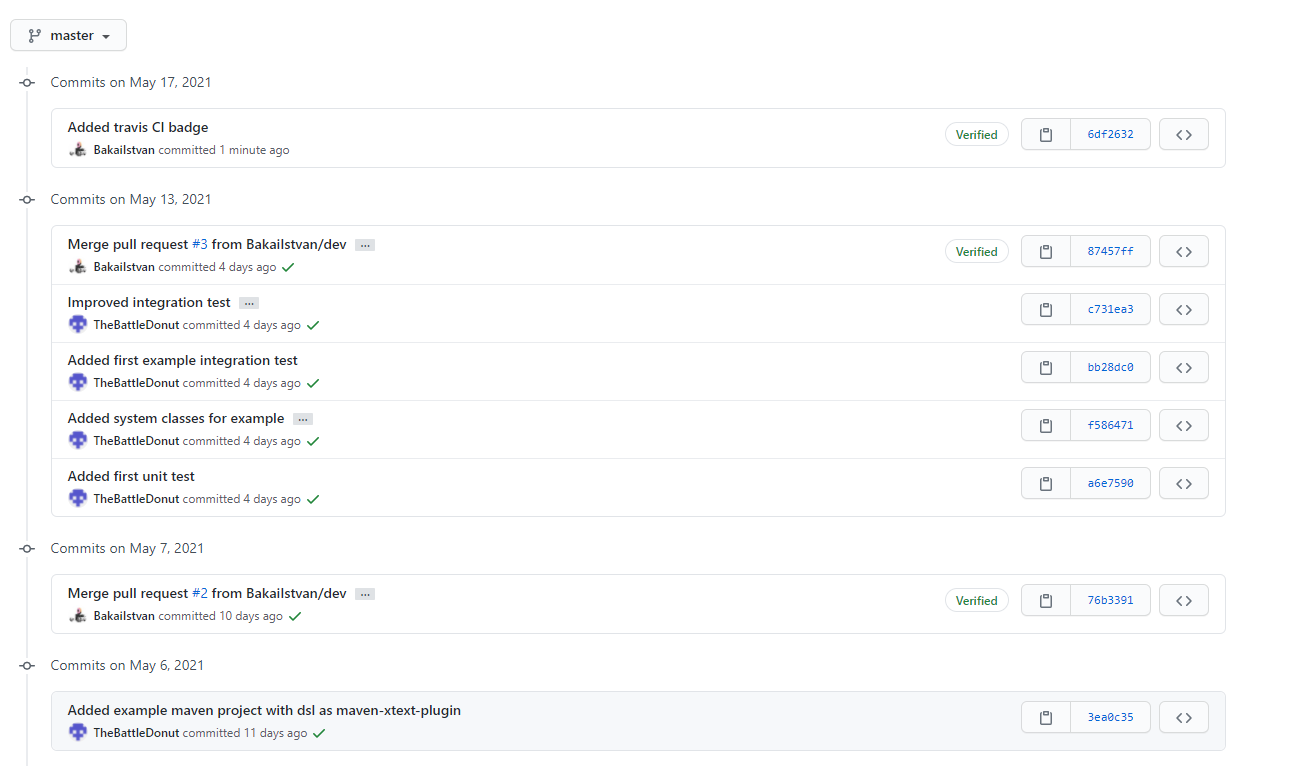
\includegraphics[width=150mm, keepaspectratio]{figures/github_ci_check.png}
    \caption{GitHub repository \textit{commit}-ok és hozzá tartozó CI \textit{check}-ek.}
    \label{commit_ci_check}
\end{figure}

\begin{figure}[!ht]
    \centering
    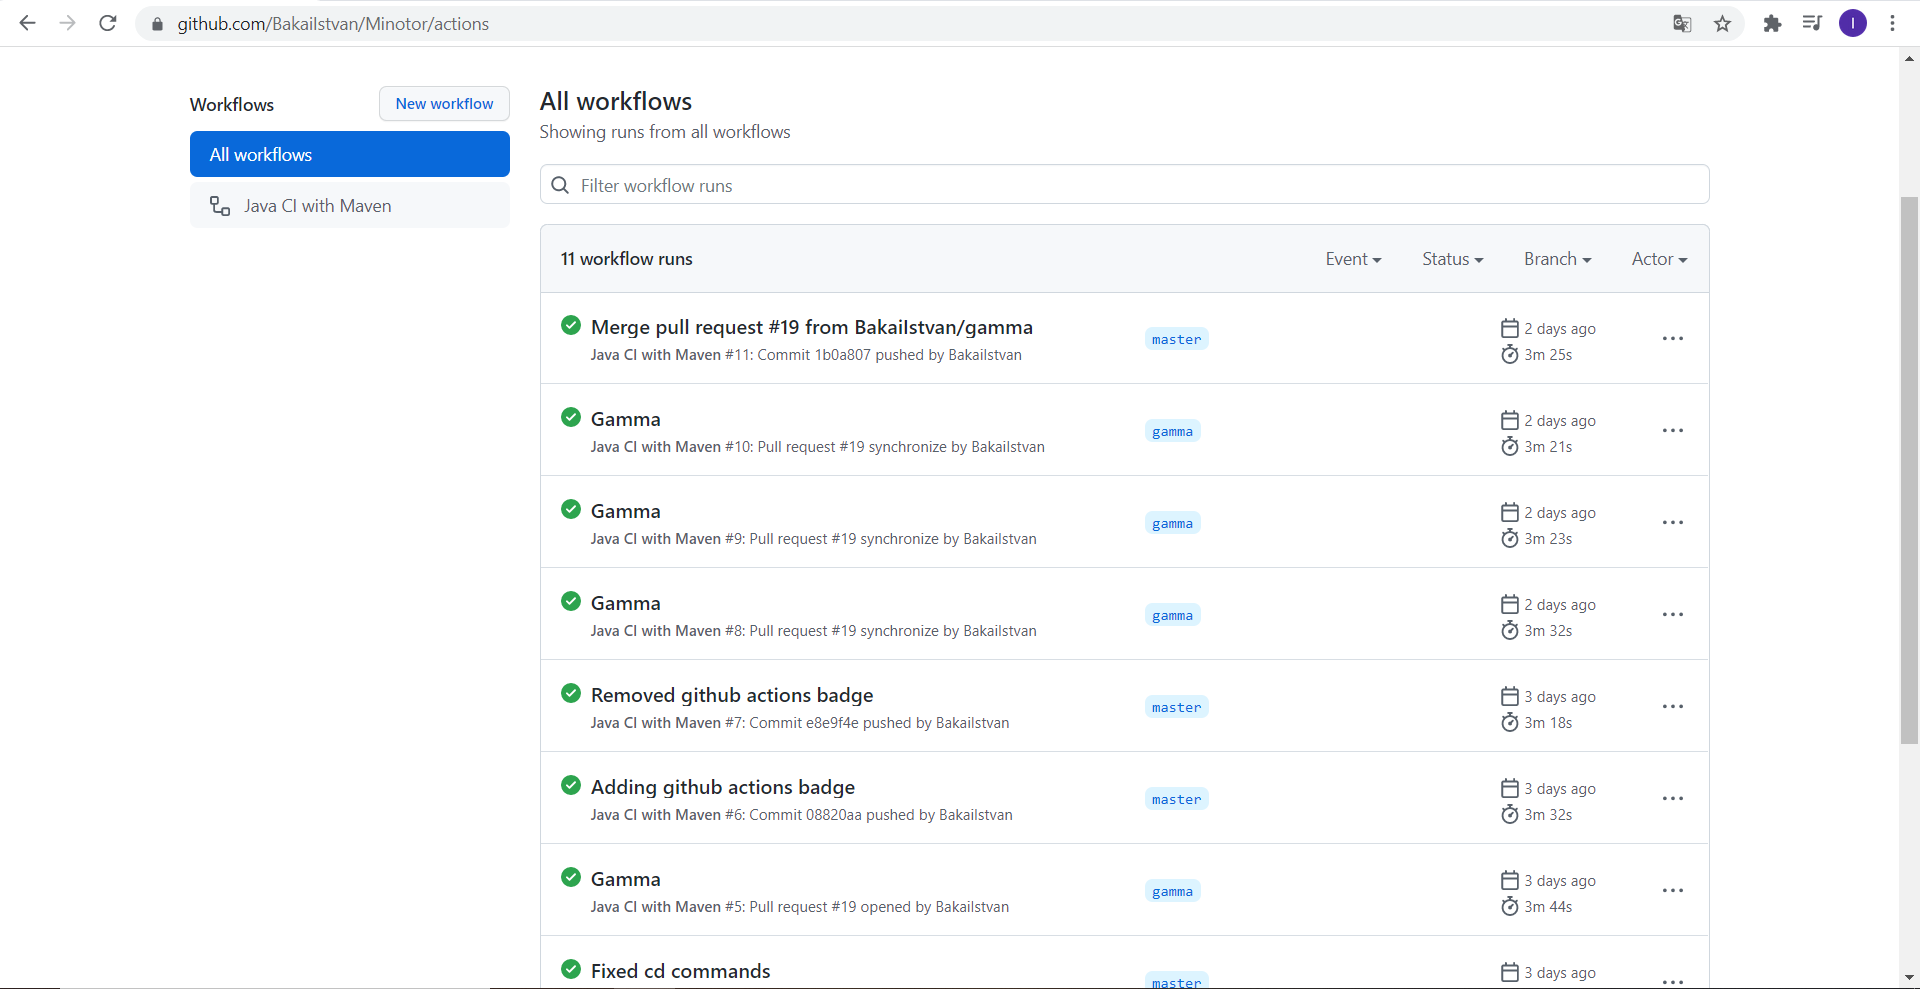
\includegraphics[width=150mm, keepaspectratio]{figures/github_ci_builds.png}
    \caption{\textit{Github Actions CI} \textit{build}-ek eredményei.}
    \label{github_actions}
\end{figure}

\begin{lstlisting}[language=java, frame=single, float=ht!, caption={\textit{Github Actions CI}-hoz tartozó \textit{.yml script}.},captionpos=b,label=ci_script]
# This workflow will build a Java project with Maven, and cache/restore any dependencies to improve the workflow execution time
# For more information see: https://help.github.com/actions/language-and-framework-guides/building-and-testing-java-with-maven

name: Java CI with Maven

on:
    push:
    branches: [ master ]
    pull_request:
    branches: [ master ]

jobs:
    build:

    runs-on: ubuntu-latest

    steps:
    - uses: actions/checkout@v2
    - name: Set up JDK 11
        uses: actions/setup-java@v2
        with:
        java-version: '11'
        distribution: 'adopt'
        cache: maven
    - name: Build with Maven
        run: mvn clean install -U
    - name: Test example project
        run: cd hu.bme.mit.dipterv.text.example; mvn clean install -U
    - name: Test mobileexample project
        run: cd hu.bme.mit.dipterv.text.mobileexample; mvn clean install -U
    - name: Test altexample project
        run: cd hu.bme.mit.dipterv.text.altexample; mvn clean install -U
    - name: Test parexample project
        run: cd hu.bme.mit.dipterv.text.parexample; mvn clean install -U
    - name: Test operatorexample project
        run: cd hu.bme.mit.dipterv.text.operatorexample; mvn clean install -U
    - name: Test gamma integration project
        run: cd hu.bme.mit.dipterv.text.gammaexample; mvn clean install -U
\end{lstlisting}

%----------------------------------------------------------------------------
\clearpage\section{Tesztesetek}
%----------------------------------------------------------------------------

Ebben a fejezetben az elkészült teszteseteket és hozzájuk tartozó tesztszcenáriókat mutatom be.
Ezeknek a teszteseteknek az a céljuk, hogy a fejezet elején ismertetett tesztelési célokat teljesítsék.
Az alfejezetek az elkészült tesztelési \textit{Maven} projekteknek felelnek meg, amelyekben bemutatom a hozzájuk tartozó tesztszcenáriókat és a szcenárióhoz tartozó teszteseteket.
Az egyszerűbb tesztszcenáriókat mutatom be először és a végén térek ki a komplexebb tesztekre.

\subsection{Egyszerű időzítési megkötéseket tartalmazó tesztszcenárió}

A tesztesetekhez tartozó szcenárió követelmény megtalálható a \ref{example_test_scenario} kódrészleten.
A szcenárióhoz tartozó diagram a \ref{example_test_scenario_diagram} ábrán látható

\begin{lstlisting}[language=java, frame=single, float=ht!, caption={Tesztesethez tartozó szcenárió szöveges leírása.},captionpos=b,label=example_test_scenario]
specification Email{

    object Computer computer;
    object Server server;

    integer timeout = 10;
    string receiver = "John";
    string subject = "Next meeting";

    clock x;

    constraint constraints {
        message logout() computer -> server;
    }

    scenario sendEmail{
        message checkEmail() computer -> computer reset x;
        required message sendUnsentEmail() computer -> server;
        fail message computerError() server -> computer;
        fail message serverError() computer -> server;
        pastConstraint {constraints} message newEmail(receiver, subject) computer -> server;
        message downloadEmail(timeout) computer -> server clockConstraint {>(x,10)};
    }
}
\end{lstlisting}

\begin{figure}[!ht]
    \centering
    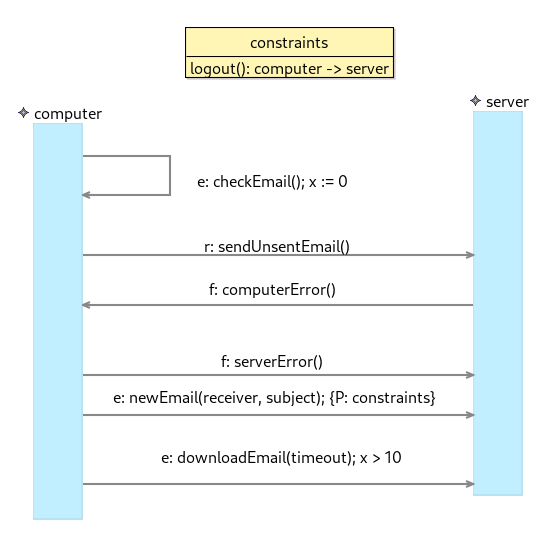
\includegraphics[width=110mm, keepaspectratio]{figures/diagramExample.png}
    \caption{Szcenárió diagram vizualizációja.}
    \label{example_test_scenario_diagram}
\end{figure}

A rendszer egy szervergépből és egy felhasználói számítógépből áll.
A szerver egy \textit{e-mail} szervert szimulál, aminek a számítógép különböző kéréseket küldhet.
Például lekérdezheti tőle a kapott \textit{e-mail}-t vagy új \textit{e-mail}-t küldhet.
A követelményben leírjuk, hogy a rendszernek mi a helyes viselkedése \textit{e-mail} küldés esetén.
Ha a computer a \textit{checkEmail} hívást használva talál elküldendő \textit{e-mail}-t az továbbítja a szervernek.
Ezt az \textit{elvárt} \textit{sendUnsentEmail} üzenet jelzi.
Ha ezt az üzenetet követően egy \textit{computerError()} üzenet jön, az a hibát jelent.
\textit{serverError()} üzenet esetén is hibát fog jelezni a monitor.
Ezt követően meg kell jelenjen a rendszer működésében a \textit{newEmail} üzenet.
Ha ehelyett \textit{logout} üzenet érkezik, az hibás működést jelent.
A \textit{newEmail} üzenetet a \textit{downloadEmail} üzenet követi.
Ezen az üzeneten van egy 10 másodperces időzítési feltétel, ami a letöltést szimulálja.

A szcenárióhoz tartozó tesztesetek a következők:
\begin{itemize}
    \item \textit{testNetworkRequirementSatisfied}, a rendszer helyes működését szimuláljuk és ellenőrizzük, hogy a generált monitor képes ezt érzékelni és jelezni.
    \item \textit{testNetworkNoErrors}, azt vizsgálja, hogy a monitor képes-e érzékelni, hogy a rendszer nem felelt meg a követelménynek.
    Itt úgy manipuláljuk a teszt rendszert, hogy lehagyjuk a letöltés részt a működésből.
    Ilyenkor a rendszer nem felel meg a követelménynek, viszont még jó állapotban marad, mert nem történt hiba.
    \item \textit{testNetworkWithErrors}, a \textit{sendUnsentEmail} üzenet után egy \textit{logout} üzenetet küldünk a monitornak és vizsgáljuk, hogy képes-e detektálni ezt a hibát.
    \item \textit{testNetworkWithNoDelay}, túl gyorsan küldjük a működés végén a \textit{downloadEmail} üzenetet és ellenőrizzük, hogy képes-e a monitor ezt a hibát érzékelni.
    \item \textit{testNetworkFirstFail}, itt a \textit{sendUnsentEmail()} után küldünk egy \textit{computerError()} üzenetet, és ellenőrizzük, hogy a monitor ezt hibának jelzi-e.
    \item \textit{testNetworkSecondFail}, itt ugyanúgy mint az előzőnél, azt ellenőrizzük, hogy a monitor a \textit{serverError()} üzenet megjelenését hibának érzékeli-e.
\end{itemize}

\begin{lstlisting}[language=java, frame=single, float=ht!, caption={\textit{testNetworkRequirementSatisfied} teszteset.},captionpos=b,label=example_test_requirement]
@Test
public void testNetworkRequirementSatisfied() {
    resetValues();
    Specification specification = new Specification();
    specification.listAutomatas();
    IClock clock = new Clock();
    IMonitor monitor = new Monitor(specification.getAutomata().get(0), clock, this);
    
    monitor.update("computer", "computer", "checkEmail", new HashMap<String, Object>());
    monitor.update("computer", "server", "sendUnsentEmail", new HashMap<String, Object>());
    monitor.update("computer", "server", "updateEmail", new HashMap<String, Object>());
    monitor.update("server", "computer", "updateAccount", new HashMap<String, Object>());
    LinkedHashMap<String, Object> hm = new LinkedHashMap<String, Object>();

    hm.put("receiver", "John");
    hm.put("subject", "Next meeting");
    monitor.update("computer", "server", "newEmail", hm);
    try {
        TimeUnit.SECONDS.sleep(11);
    } catch (InterruptedException e) {
        e.printStackTrace();
    }
    monitor.update("computer", "server", "downloadEmail", Map.of("timeout", 10));
    
    Assertions.assertTrue(monitor.goodStateReached());
    Assertions.assertTrue(monitor.requirementSatisfied());
    Assertions.assertTrue(requirementSatisfied);
    Assertions.assertFalse(errorDetected);
}
\end{lstlisting}

A \ref{example_test_requirement} kódrészlet \textit{testNetworkRequirementSatisfied} teszteset implementációját tartalmazza.
Először létrehozzuk a monitort és átadjuk neki a szöveges leírás alapján generált időzített automatát.
Ezután végig megyünk az esemény szekvencián, amelyet a monitornak az \textit{update()} függvény segítségével juttatunk el.
A teszteset végén pedig összevetjük a monitor kimenetét az elvárt kimenettel.
Például ennél a tesztesetnél a monitornak azt kell jeleznie, hogy a rendszer jó állapotban van, megfelelt a követelménynek és nem történt hiba.

%----------------------------------------------------------------------------
\clearpage\subsection{Többféle üzenetet és megkötést tartalmazó egyszerű tesztszcenárió}
%----------------------------------------------------------------------------

\begin{lstlisting}[language=java, frame=single, float=ht!, caption={Második tesztesethez tartozó szcenárió.},captionpos=b,label=second_scenario_test]
    specification Photo{

        object User user;
        object Device device;
        object Database db;

        clock x;

        constraint error {
            message closeApp() user -> device;
        }

        scenario playlist_generation{
            message openApp() user -> device reset x;
            message accessWebcam() device -> device clockConstraint {<=(x, 5)} reset x;
            required futureConstraint {error} message getPhoto() device -> user;
            fail message cameraOffline() user -> device;
            required strict message retrieveMood() device -> db;
            required message retrieveMusic() device -> db;
            strict message generatePlaylist() db -> device clockConstraint {<(x, 15)};
        }
    }
\end{lstlisting}

\begin{figure}[!ht]
    \centering
    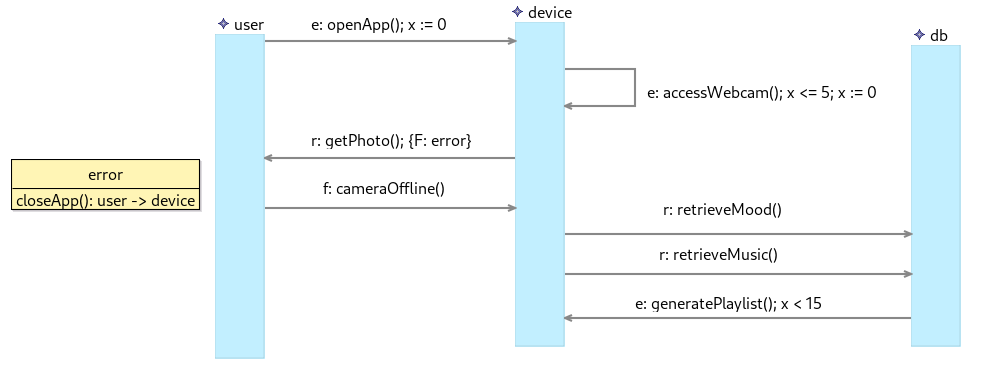
\includegraphics[width=160mm, keepaspectratio]{figures/diagramMobileExample.png}
    \caption{Második szcenárióhoz tartozó diagram vizualizációja.}
    \label{second_visualization}
\end{figure}

A tesztrendszerünk egy zene lista generáló alkalmazás, ami egy felhasználót, mobileszközt és adatbázist tartalmaz.
A felhasználó "\textit{kedve}" alapján generálja a listát, amit az arckifejezése alapján határoz meg.
A követelményben a rendszer alap működése van leírva egészen az elejétől, amikor a felhasználó megnyitja az alkalmazást.
A követelmény leírás megtekinthető a \ref{second_scenario_test} kódrészleten és a hozzá tartozó vizualizáció a \ref{second_visualization} ábrán.

A szcenárióhoz tartozó tesztesetek a következők:

\begin{itemize}
    \item testMobileRequirementSatisfied, a követelmény teljesülését ellenőrizzük.
    \item testMobileFutureConstraint, azt vizsgáljuk, hogy a monitor hibát jelez-e, ha megkötésbeli üzenet érkezik.
    \item testMobileFutureConstraintEarly, azt vizsgáljuk hogy a monitor hibát jelez-e, ha a megkötésbeli üzenet az üzenet szekvencia elején érkezik.
    \item testMobileWithError, a monitor hibát jelez-e, amikor a \textit{cameraOffline()} üzenet érkezik.
    \item testMobileWithDelay, késleltetjük az \textit{accessWebcam()} üzenet megérkezését úgy, hogy az időzítési feltétel teljesüljön és vizsgáljuk, hogy a monitor ezt helyesen kezeli-e.
    \item testMobileWithTooMuchDelay, késleltetjük az \textit{accessWebcam()} üzenetet  az időzítési feltételt elrontva és azt várjuk el, hogy a monitor ezt hibának jelezze.
    \item testMobileMissingRequiredMessage, vizsgáljuk hogy a monitor hibát jelez-e, ha nem kapja meg az \textit{retrieveMood()} elvárt üzenetet.
    \item testMobileRequiredEventually, a monitor helyes működést kell jelezzen, ha az elvárt üzenetet megkapja, még ha más üzenetek is előjönnek ez alatt.
    \item testMobileRequiredNotReceived, a monitor nem érzékeli a \textit{retrieveMusic()} üzenetet, ezért hibát kell jelezzen.
\end{itemize}

A tesztesetek a monitor hibadetektáló képeségét tesztelik.
A \textit{testMobileWithDelay} és \textit{testMobileWithTooMuchDelay} tesztesetek az \textit{x <= 5} időzítési feltétel beteljesülését ellenőrzik.
A \textit{testMobileWithDelay} tesztesetben 5 másodperces késleltetéssel küldjük az \textit{accessWebcam} üzenetet, míg a másiknál 6 másodperces késleltetéssel.
Az első esetben a monitornak helyes működést kell érzékelnie, a következőben pedig hibás működést.

%----------------------------------------------------------------------------
\subsection{Alt operátort tartalmazó tesztszcenárió}
%----------------------------------------------------------------------------

A tesztszcenárióhoz tartozó rendszerünk egy banki rendszer.
A szcenárió megtalálható az \ref{thrid_test_scenario} kódrészleten és a hozzá tartozó vizualizáció a \ref{third_visualisation} ábrán látható.

\begin{lstlisting}[language=java, frame=single, float=ht!, caption={Alt operátort tartalmazó tesztszcenárió.},captionpos=b,,label=thrid_test_scenario]
specification Bank {

    object UserInterface ui;
    object ATM atm;
    object BankDB db;

    bool success = true;

    constraint b {
        message logout() ui->atm;
    }

    scenario transaction {
        message login(success) ui->atm;

        alt (equals(success, true)) {
            pastConstraint {b} message wReq() ui->atm;
            message uDB() atm->db;
        } (equals(success, false)) {
            message loginUnsuccessful() ui->atm;
            required message lockMachine() atm->ui;
        }
    }
}
\end{lstlisting}

\begin{figure}[!ht]
    \centering
    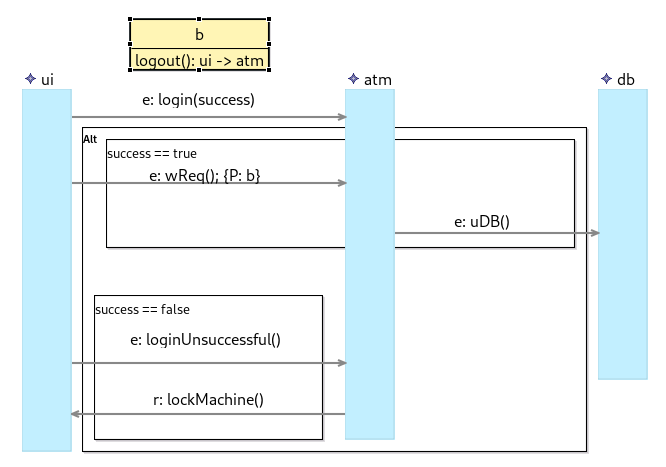
\includegraphics[width=120mm, keepaspectratio]{figures/diagramAltExample.png}
    \caption{Alt operátort tartalmazó szcenárió diagram}
    \label{third_visualisation}
\end{figure}

A rendszer egy felhasználói felületből, \textit{ATM}-ből és banki adatbázisból áll.
A követelményünkben két lehetséges működést írunk le.
A \textit{success} paraméter jelzi, hogy melyik működés a helyes.
A szcenárióhoz tartozó tesztesetek a következők:

\begin{itemize}
    \item testBankMonitorPassing, az operátorban levő első ágnak megfelelően szimuláljuk a rendszer működését és elvárjuk, hogy a monitor helyes működést jelezzen.
    \item testBankMonitorFailing, a monitornak hibát kell jeleznie, ha az operátor első ágától eltér a működés.
    \item testBankMonitorFalseCasePassing, a monitornak helyes működést kell jeleznie, ha a rendszert úgy szimuláljuk ahogy az operátor második ágában le van írva.
    \item testBankMonitorFalseCaseFailing, a monitor hibát jelez, ha nem az operátor második ága szerint működik a rendszer.
\end{itemize}

A tesztesetekkel azt vizsgáljuk, hogy a monitor képes-e a helytelen ág lefutását hibának érzékelni és a helyes viselkedés esetén detektálni a követelmény teljesítését.

%----------------------------------------------------------------------------
\subsection{Par operátort tartalmazó tesztszenárió}
%----------------------------------------------------------------------------

\begin{lstlisting}[language=java, frame=single, float=ht!, caption={Par operátort tartalmazó tesztszcenárió.},captionpos=b]
specification Email {
    object Computer computer;
    object Server server;

    constraint constraints{
        message logout() computer -> server;
    }

    scenario email {
        par {
            case checkEmail {
                message checkEmail() computer -> computer;
            }

            case newEmail {
                pastConstraint {constraints} message newEmail() computer -> server;
            }
        }
    }
}
\end{lstlisting}

\begin{figure}[!ht]
    \centering
    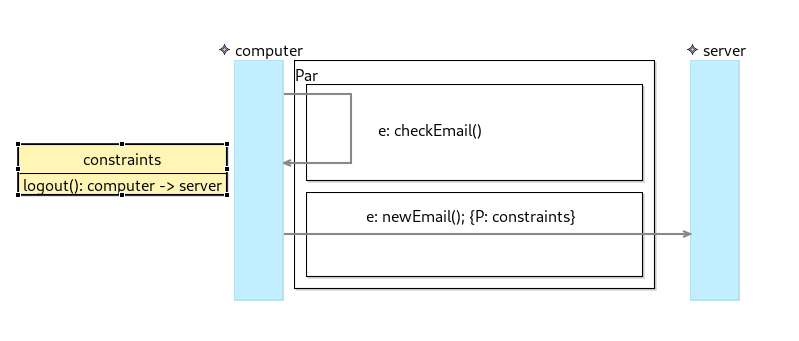
\includegraphics[width=150mm, keepaspectratio]{figures/diagramParExample.png}
    \caption{Par operátort tartalmazó szcenárió diagram.}
\end{figure}

Ehhez a tesztszcenárióhoz az első szcenárióban lévő teszt rendszert használtam fel.
A szcenárióhoz tartozó tesztesetek a következők:

\begin{itemize}
    \item testNetworkRequirementSatisfied, az első permutáció szerint működtetjük a szimulált rendszert, a monitornak helyes működést kell jeleznie.
    \item testNetworkOtherRequirementSatisfied, a második permutáció szerint működtetjük a rendszert, a monitornak helyes működést kell jeleznie.
\end{itemize}

Azt vizsgáljuk, hogy a monitor képes-e mindkét permutáció esetén érzékelni a követelmény teljesülését.

%----------------------------------------------------------------------------
\subsection{Komplex tesztszcenárió loop és alt operátorokkal}
%----------------------------------------------------------------------------

\begin{lstlisting}[language=java, frame=single, float=ht!, caption={Komplex teszteset szcenáriója.},captionpos=b,label=test_complex_scenario]
specification Connection {

    object Computer computer;
    object Server server;

    string receiver = "John";
    string subject = "Next Meeting";
    bool success = false;

    clock x;
    clock y;

    constraint logout {
        message logout() computer -> server;
    }

    constraint delete {
        message deleteEmail(subject) computer -> server;
    }

    scenario authentication {
        loop (1, 3) {
            message login(success) computer -> computer reset x;
            pastConstraint {logout} message attemptLogin() computer -> server reset y;
        }

        alt (equals(success, true)) {
            message checkEmail() computer -> server clockConstraint {<(x, 2)};
            required futureConstraint {delete} message newEmail(receiver, subject) computer -> server reset x;
        } (equals(success, false)) {
            required message logoutUser() server -> computer clockConstraint {>(y, 3)};
            message lockComputer() server -> computer reset y;
        }
    }
}
\end{lstlisting}

\begin{figure}[!ht]
    \centering
    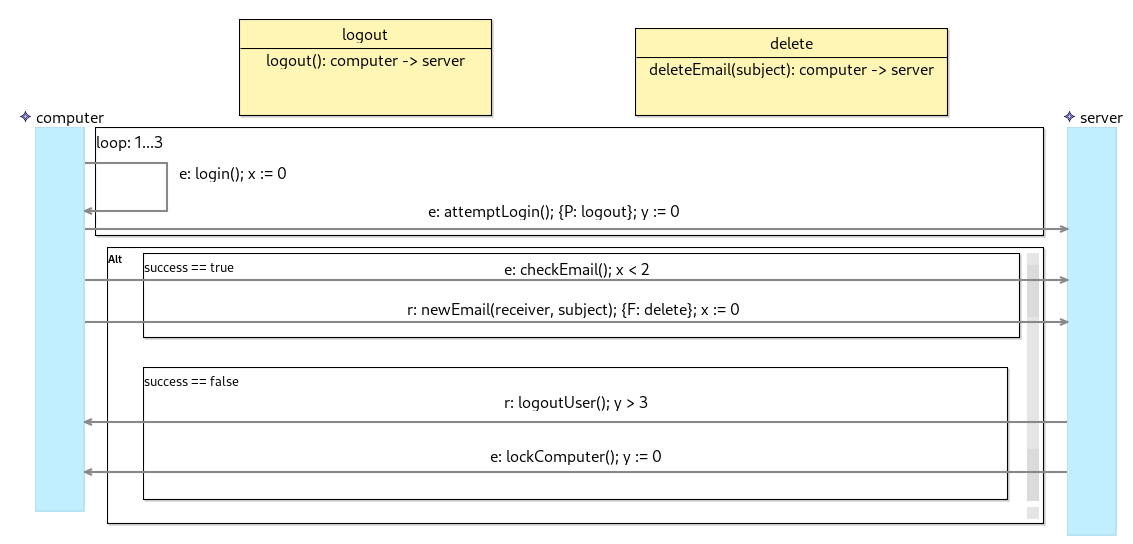
\includegraphics[width=160mm, keepaspectratio]{figures/diagramOperatorExample.png}
    \caption{Komplex szcenárió diagram vizualizációja.}
    \label{test_complex_diagram}
\end{figure}

Ebben a tesztszcenárióban olyan szcenáriók támogatását teszteljük, amelyekben több operátor is megjelenik.
A tesztesethez tartozó szcenárió a \ref{test_complex_scenario} kódrészletben található meg és a diagram vizualizációja a \ref{test_complex_diagram} ábrán látható.
Ezen kívül vizsgáljuk, hogy a generált monitor képes-e több óraváltozó kezelésére is.

A szcenárióban a \textit{loop} operátort használva egy felhasználó többszörös bejelentkezési próbálkozását írjuk le.
Utána egy \textit{alt} operátorral mondjuk meg, hogy minek kell történnie sikeres vagy sikertelen bejelentkezés esetén.

A tesztszcenárióhoz tartozó tesztesetek:
\begin{itemize}
    \item testNetworkRequirementSatisfied, a követelmény teljesülését ellenőrizzük.
    \item testNetworkRequirementSatisfiedTwice, a követelménynek akkor is teljesülnie kell, ha a \textit{loop} operátorban lévő üzenetek kétszer egymás után jelennek meg.
    \item testNetworkRequirementSatisfiedThreeTimes, az üzenetek háromszor egymás után jelennek meg.
    \item testNetworkRequirementSatisfiedFourTimes, a monitornak hibát kell jeleznie, ha négyszer érzékeli az üzeneteket, melyek a \textit{loop} operátorban vannak, hiszen az meghaladja a maximumot.
    \item testNetworkAltTrueCase, a monitor hibát jelez, ha úgy működtetjük a szimulált rendszer, hogy az \textit{alt} operátor igaz ágában lévő üzenetek jelenjenek meg.
    \item testNetworkAltTrueCaseSatisfied, a monitor helyes működést kell jelezzen, ha ugyanúgy szimuláljuk a rendszer működését, mint az előző tesztesetben.
    \item testNetworkLogoutTooFast, ha túl gyorsan érkezik meg a \textit{logoutUser()} üzenet, akkor a monitornak hibát kell jeleznie.
    \item testNetworkLogoutConstrait, ha olyan üzenet érkezik, amely a megkötésben szerepel, akkor a monitornak hibát kell jeleznie.
\end{itemize}

A teszteseteket úgy állítottam össze, hogy ellenőriztem mind a monitor hibadetektáló képességét, mind a helyes működés detektálását.

\clearpage\section{Tesztelés összefoglaló}

A \ref{tab:table1} táblázat mutatja be a tesztelés eredményét.
Sikerült az összes tesztelési célnak megfelelni, emellett biztosítani a szisztematikus ellenőrzést.
Minden teszt sikeresen lefutott.

\begin{longtable}{|p{0.1428\linewidth}|p{0.1428\linewidth}|p{0.1428\linewidth}|p{0.1428\linewidth}|p{0.1428\linewidth}|p{0.1428\linewidth}|}
\hline
\textbf{Tesztelési célok} & \textbf{Egyszerű tesztszcenárió} & \textbf{Több üzenetet tartalmazó tesztszcenárió} & \textbf{Alt operátort tartalmazó tesztszcenárió} & \textbf{Par operátort tartalmazó tesztszcenárió} & \textbf{Komplex tesztszcenárió}\\
\hline
Egyszerű üzenet megjelenése & X & X & X & X & X\\
\hline
Elvárt üzenet megjelenése & X & X & X & - & X\\
\hline
Nem kivánt (fail) üzenet megjelenése & X & X & - & - & -\\
\hline
Strict üzenet tesztelése & - & X & - & - & -\\
\hline
Időzítési feltételek tesztelése & X & X & - & - & X\\
\hline
Past megkötés tesztelése & X & - & X & X & X\\
\hline
Future megkötés tesztelése & - & X & - & - & X\\
\hline
Alt operátor tesztelése & - & - & X & - & X\\
\hline
Par operátor tesztelése & - & - & - & X & -\\
\hline
Loop operátor tesztelése & - & - & - & - & X\\
\hline
Több operátort tartalmazó szenárió tesztelése & - & - & - & - & X\\
\hline
Egymást követő elvárt üzenetek & - & X & - & - & -\\
\hline
Egymást követő fail üzenetek & X & - & - & - & -\\
\hline
Egyszerű üzenet tesztelése & X & X & X & X & X\\
\hline
Több óraváltozó & - & - & - & - & X\\
\hline
Elvárt után fail üzenet & X & - & - & - & -\\
\hline
Fail után elvárt üzenet & - & X & - & - & -\\
\hline
\caption{Összefoglaló táblázat}
\label{tab:table1}
\end{longtable}